\documentclass[12pt, a4paper]{article}
\usepackage[top=1.0in, bottom=1.0in, left=0.8in, right=0.8in]{geometry}

\setlength{\parskip}{\baselineskip}%
\setlength{\parindent}{0pt}%
\usepackage{bookmark}
\usepackage[]{graphicx}
\usepackage{enumitem}
\usepackage{amsmath}
\usepackage{relsize}
\usepackage{cprotect}
\usepackage{amsmath, amsfonts}
\usepackage{siunitx}
\usepackage{mathrsfs}
\usepackage{framed}
\usepackage{enumitem}
\usepackage{tikz}
\usepackage{circuitikz}
\usepackage{float}
\usepackage[english]{babel}
\usepackage{blindtext}

\newlist{notes}{enumerate}{1}
\setlist[notes]{label=\textbf{Note:} ,leftmargin=*}

\newlist{hints}{enumerate}{1}
\setlist[hints]{label=\textbf{Hint:} ,leftmargin=*}

\usepackage{xcolor}
\usepackage{color}
\definecolor{com1}{RGB}{125,125,125}
\definecolor{comment}{RGB}{140,115,115}
\definecolor{numbering}{rgb}{0.2,0.2,0.2}
\definecolor{key}{RGB}{0,0,180}
\definecolor{in}{RGB}{0,100,0}
\definecolor{out}{RGB}{100,30,30}
\definecolor{bg}{RGB}{245,245,245}
\definecolor{bgLight}{RGB}{250,250,250}
\definecolor{string}{RGB}{0,150,0}

\usepackage{hyperref}
\hypersetup{
    colorlinks=true,
    linkcolor=blue,
    filecolor=magenta,      
    urlcolor=blue,
}
\urlstyle{same}

\usepackage{listings}

\lstdefinestyle{py_code}{ %
    backgroundcolor=\color{bg},      % choose the background
    basicstyle=\ttfamily\small,		      % fonts
    breakatwhitespace=false,         % automatic breaks at whitespace ?
    breaklines=true,                 % sets automatic line breaking
    captionpos=b,                    % caption-position - bottom
    commentstyle=\itshape\color{comment},    % comment style
    extendedchars=true,              % use non-ASCII
    frame=single,	                   % single frame around the code
    keepspaces=true,                 % keeps spaces in text
    keywordstyle=\bfseries\color{key},% keyword style
    language=Python,                 	  % the language of the code
    morekeywords={Null},       % add more keywords to the set
    numbers=left,                    % line_numbers (none, left, right)
    numbersep=10pt,                  % line_no - code dist
    numberstyle=\footnotesize\color{numbering}, % line_no style
    rulecolor=\color{black},         % frame_color [!always set]
    showspaces=false,                % show spaces everywhere
    showstringspaces=false,          % 
    showtabs=false,                  % 
    stepnumber=1,                    % step b/w two line-no
    stringstyle=\color{string},     % string literal style
    tabsize=2,	                       % sets default tabsize to 2 spaces
    title=\lstname,                  % show the filename
    escapeinside={(*}{*)},			  % escape from style inside (* *)
    xleftmargin=\parindent,
    belowskip=-1.3 \baselineskip,
    aboveskip=1.0 \baselineskip,
    columns=fullflexible,
    xleftmargin=0.15in,
}
\lstnewenvironment{py_code}
{\lstset{style=py_code}}
{}

\lstdefinestyle{psudo}{ %
    backgroundcolor=\color{bgLight},   % choose the background
    basicstyle=\ttfamily\small,		      % fonts
    breakatwhitespace=false,         % automatic breaks at whitespace ?
    breaklines=true,                 % sets automatic line breaking
    captionpos=b,                    % caption-position - bottom
    commentstyle=\itshape\color{com1},          % comment style
    extendedchars=true,              % use non-ASCII
    keepspaces=true,                 % keeps spaces in text
    language=C,                 	  % the language of the code
    morekeywords={type,NULL, True, False},       % add more keywords to the set
    showspaces=false,                % show spaces everywhere
    showstringspaces=false,          % 
    showtabs=false,                  % 
    tabsize=2,	                       % sets default tabsize to 2 spaces
    title=\lstname,                  % show the filename
    escapeinside={(*}{*)},			  % escape from style inside (* *)
    belowskip=-1.8 \baselineskip,
    aboveskip=0.9 \baselineskip,
    columns=fullflexible,
    xleftmargin=0.2in,
    frame=tb,
    framexleftmargin=16pt,
    framextopmargin=6pt,
    framexbottommargin=6pt, 
    framerule=0pt,
}

\lstnewenvironment{psudo}
{\lstset{style=psudo}}
{}

\graphicspath{ ./ }

\title{\textbf{EE2703 : Applied Programming Lab \\ Assignment 9 \\ Spectra of non-periodic signals}} 
\author{Chagari Koushal Kumar Reddy \\ EE20B023} % Author name

\date{\today} % Date for the report

\begin{document}		

\maketitle % Insert the title, author and date
\clearpage

\tableofcontents
\clearpage

\section{Aim}
The aim of this assignment is to:
\begin{enumerate}
    \item Learn how DFT is used to analyze spectra of non-periodic DT signals.
    \item Analyze spectra of non-periodic sinusoidal DT signals using and without using Hamming window.
    \item Estimate the frequency and initial phase of a single sinusoid by finding its DFT and analyzing it.
    \item Find the DFT of a chirped signal and also plot DFTs fo different segments of it to see how the frequency components change with time.
\end{enumerate}
\section{Theory}
\subsection{DFT of signals with discontinuities}
The DFT and inverse DFT equations are:
\begin{equation*}
    a[k] = \sum_{n=0}^{N-1}x[n]e^{-j\frac{2\pi}{N}kn}
\end{equation*}
\begin{equation*}
    x[n] = \sum_{k=0}^{N-1}\frac{a[k]}{N}e^{j\frac{2\pi}{N}kn}
\end{equation*}
As we can see, both the equations are inherently periodic with period as N samples. Hence both the functions $x[k]$ and $a[k]$ are periodic. Now let's say the samples which are at the ends of one period of signal $x[n]$ are periodic. Now let's say the samples which are at the ends 
in one period of signal $x[n]$ have a big difference. Now, there is a discontinuity in the signal. Because of this discontinuity, the spectrum of the signal will contain fourier coefficients which will decay as $\frac{1}{\omega}$. So even if the samples are part of a sinusoid, the $\frac{1}{\omega}$ decay will be present if the samples at the end are not so close.

An example for this is $x[n]=\sin{\sqrt{2}t}$ with the period as $2\pi$. Even though the signal is periodic, the time range we took is not a period of it. So the periodic extension for period $T = 2\pi$ will not produce $\sin(\sqrt{2}t)$ but a different signal. Hence the DFT will also not have two impulses but a contionously decreasing spectrum.
\begin{figure}[H]
    \centering
    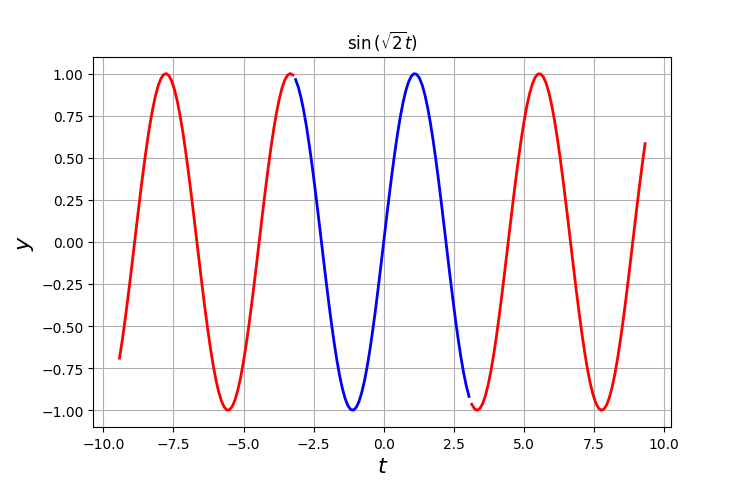
\includegraphics[scale = 0.8]{Figure_1.png}
    \label{fig:sample}
\end{figure}
\begin{center}
    This is the original signal $\sin(sqrt{2}t)$
\end{center}

\begin{figure}[H]
    \centering
    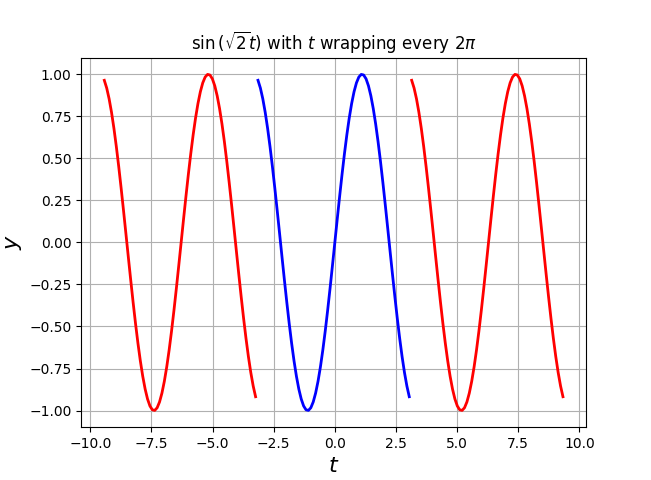
\includegraphics[scale = 0.8]{Figure_2.png}
    \label{fig:sample}
\end{figure}
\begin{center}
    Signal whose first period ($T = 2\pi$) contains samples of $\sin(\sqrt{2}t)$ and the remaining samples are periodic repetitions of the first-period samples
\end{center}
The singal of this signal will be:
\begin{figure}[H]
    \centering
    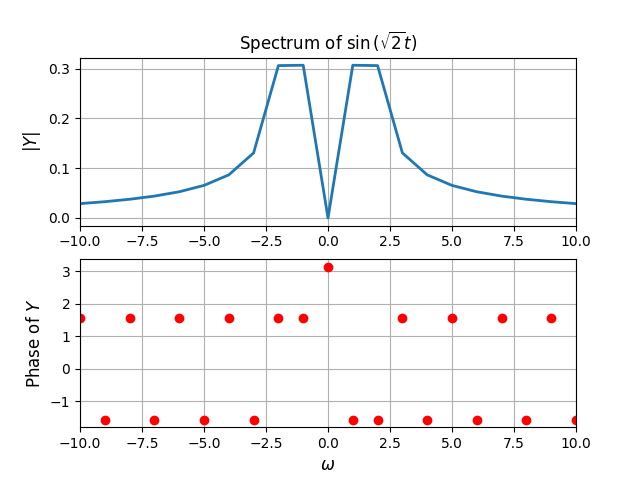
\includegraphics[scale = 0.8]{Figure_3.png}
    \label{fig:sample}
\end{figure}
\begin{center}
    DFT of $\sin(\sqrt{2}t)$ for $T = 2\pi$ and $N=64$
\end{center}
As we can see, we have peaks around $\sqrt{2}$ but they are not impulses. Rather, we have a continuous spectrum which to have a $\frac{1}{\omega}$. But, first of all where does this decay come from?
\subsection{Gibbs Phenomena}
Gibbs phenomena occurs when a signal contains discontinuities. We know sinusoids are continuous signals. Hence, when we try to model a discontinous function as sum (or) integral sinusoids to achieve that discontinuity. Hence, the spectrum will decay slowly and won't even become zero after some frequency, i.e., spectrum won't be bandlimited. Let us take the example of a periodic linear ramp with period $2\pi$. It's equation is defined as:
\begin{equation*}
    x(t) = t \forall t \in [-\pi,\pi)
\end{equation*}
and this segment is periodically repeated to get the periodic linear ramp. Clearly, we have discontinuities at $t = n\pi$ where $n$ is an integer. Now, the fourier series representation of this signal would be:
\begin{equation*}
    x(t) = 2(\frac{\sin(t)}{1} - \frac{\sin(2t)}{2} + \frac{\sin(3t)}{3} \ldots )
\end{equation*}
The spectrum of this signal on a dB-dec plot is as follows:
\begin{figure}[H]
    \centering
    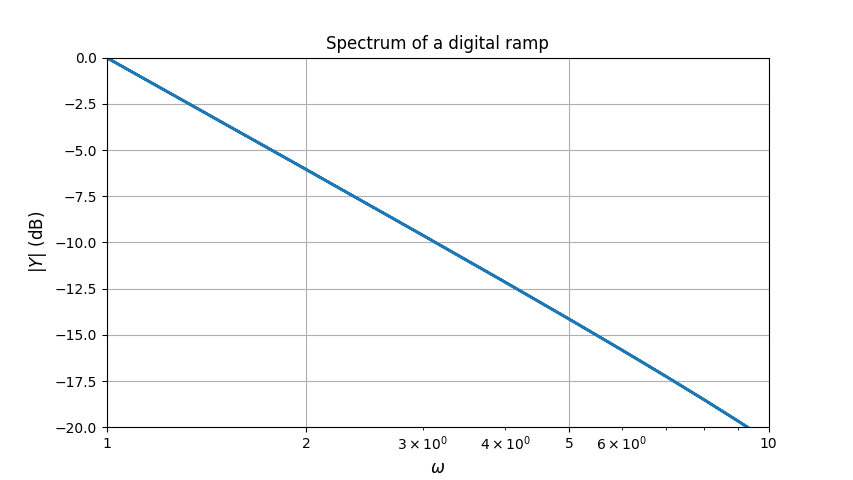
\includegraphics[scale = 0.8]{Figure_4.png}
    \label{fig:sample}
\end{figure}
\begin{center}
    The spectrum decays linearly with respect to $\omega$ on the dB-dec plot indicatign a $\frac{1}{\omega}$ decay as expected
\end{center}
\subsection{Hamming Window}
To avoid discontinuities, we use a Hamming Window. This Hamming Window is another DT signal which will be multiplied with the original signal. This window signal will be high inside the period and nearly zero at the edges.
Hence the edge discontinuities are dampened whereas the signal within the bulk of the period is preserved. An example for a Hamming Window is:
\begin{equation*}
    w[n] = 0.54 + 0.46\cos(\frac{2\pi n}{N-1}) \forall 0 \leq n < N
\end{equation*}
and this signal is also periodically repeated. The new refined signal after the multiplication with the window signal is plotted below:
\begin{figure}[H]
    \centering
    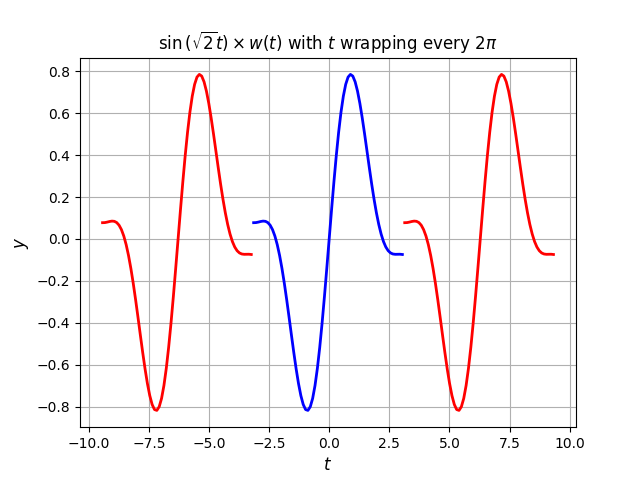
\includegraphics[scale = 0.8]{Figure_5.png}
    \label{fig:sample}
\end{figure}
\begin{center}
    The period is still maintained as $2\pi$ and the frequency as $\sqrt{2}$. But now teh discontinuities are reduced because of the multiplication with the window signal
\end{center}
Now let us plot the DFT of this refined signal. The DFT of this new signal will be circular convolution of the DFTs of the original signal and the window signal (Multiplication in time domain leads to convolution in the frequency domain and vice-versa):
\begin{equation*}
    G_{k} = \sum_{n=0}^{N-1}F_{n}W_{k-n}
\end{equation*}
Hence we expect the $\frac{1}{\omega}$ decay to have vanished since the DFT of $w[n]$ only contains components at DC and $\omega = \pm 1$. Hence we can write:
\begin{equation*}
    G_{k} = F_{k}W_{0} + F_{k+1}W_{-1} + F_{k-1}W_{1}
\end{equation*}
Clearly this summation does not exist for all values of $k$ but only at those values of $k$ where the DFT of $x[n]$ is high. So, the DFT of the refined signal will be:
\begin{figure}[H]
    \centering
    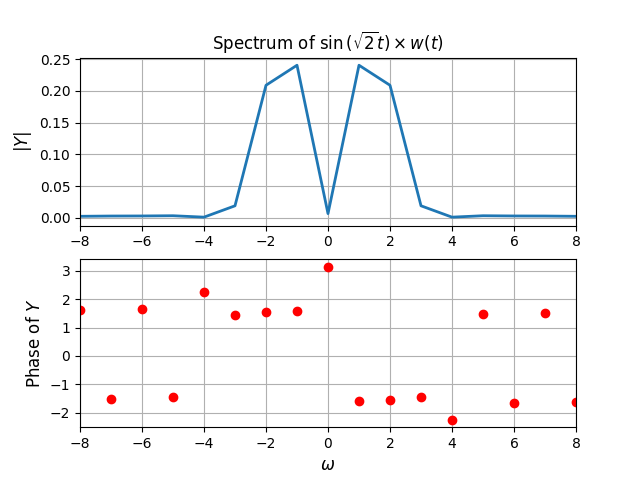
\includegraphics[scale = 0.8]{Figure_6.png}
    \label{fig:sample}
\end{figure}
\vspace*{-0.5cm}
\begin{center}
    The DFT is not accurate but much better when compared to the DFT of the unrefined signal
\end{center}
\vspace*{-0.5cm}
We got rid of the $\frac{1}{\omega}$ decay but the peaks are still broad. We really cannot do anything about it because of the Hamming Window. The convolution sum doesn't decay instantly. It exists for $k$ values which are around $\sqrt{2}$ and then only becomes zero. That's why we have a broad peak even after windowing is done.

One improvement which we can do to get an relatively accurate pattern is to increase the resolution, i.e., increase the time range (or period) $T$ for which it is calculated. Let's assume now the signal runs from $[-4\pi,4\pi)$ with $N=257$. The signal will look like this:
\vspace*{-0.5cm}
\begin{figure}[H]
    \centering
    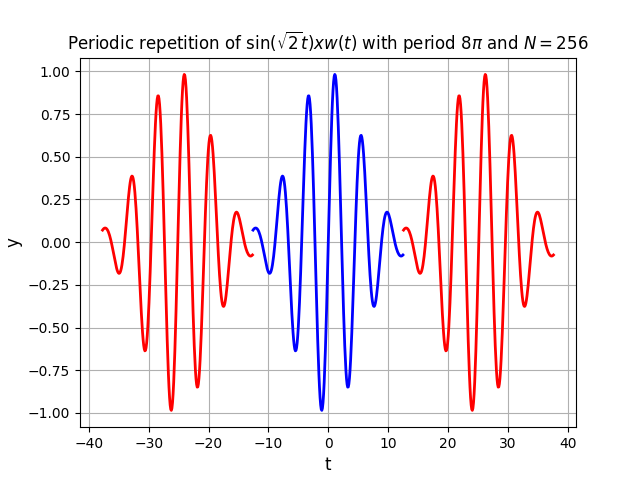
\includegraphics[scale = 0.75]{Figure_7.png}
    \label{fig:sample}
\end{figure}
\begin{center}
    Here the period is $8\pi$ and $N=257$. Again, we periodically repeat the first period to get the whole periodic signal
\end{center}
DFT of this signal is shown below:
\begin{figure}[H]
    \centering
    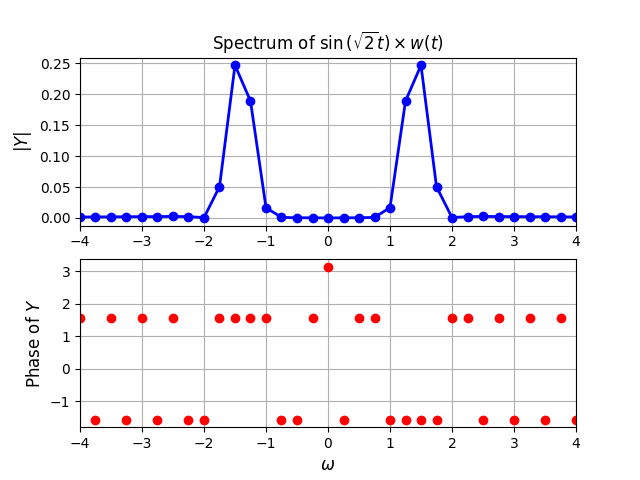
\includegraphics[scale = 0.8]{Figure_8.png}
    \label{fig:sample}
\end{figure}
\begin{center}
    The DFT is still broad but definitely better than the previous DFT plot
\end{center}
\section{Assignment}
\subsection{Spectrum of $\cos^{3}(t)$}
We know:
\begin{equation*}
    \cos^{3}(\omega_{o}t) = 0.75\cos(\omega_{o}t) + 0.25\cos(3\omega_{o}t) 
\end{equation*}

\begin{equation*}
    \cos^{3}(\omega_{o}t) = 0.375e^{j\omega_{o}(t)} + 0.375e^{-j\omega_{o} t} + 0.125e^{j3\omega_{o}t} + 0.125e^{-j3\omega_{o}t}
\end{equation*}

Hence we would expect 4 sharp peaks at the given frequencies. However, in this problem, our time range is a multiple of $2\pi$ which is clearly not a period since $\omega_{o}=0.86$. Hence the periodic repetition won't be $\cos^{3}(0.86t)$ and we will be facing the same problems we had with $\sin(\sqrt(2)t)$. So, our DFT plot will be continuous with broad peaks at the given frequencies. The DFT plot for period time range $[-4\pi,4\pi)$ and $N=256$ is given below:
\begin{figure}[H]
    \centering
    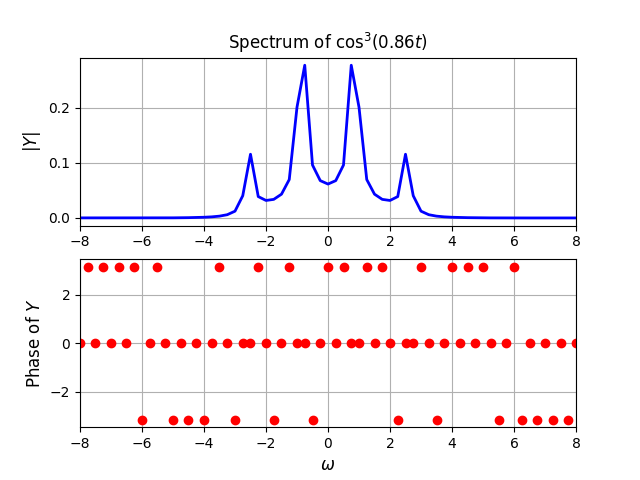
\includegraphics[scale = 0.8]{Figure_9.png}
    \label{fig:sample}
\end{figure}
\begin{center}
    This is the DFT plot without the hamming window
\end{center}
\begin{figure}[H]
    \centering
    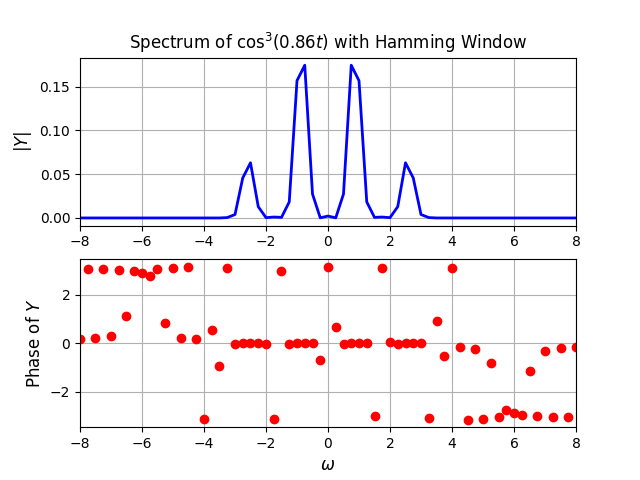
\includegraphics[scale = 0.8]{Figure_10.png}
    \label{fig:sample}
\end{figure}
\begin{center}
    The DFT plot is better when the Hamming Window is introduced. However, the peaks are still broad because of the reasons discussed in section 2.3
\end{center}
\subsection{Estimation of frequency and initial phase of a sinusoid using DFT:}
DFT plotting could also be used to find the frequency and initial phase of a sinusoidal signal. For estimating $\omega$, we use the following formula since the peak is broad and the frequency is difficult to see:
\begin{equation*}
    \omega_{o} = \frac{\sum |Y|^{p}\omega}{\sum |Y|^{p}}
\end{equation*}
that is we are taking the weighted average of the frequencies with the weights being the magnitude of the signal at the frequency. Also the value of p was chosen as $3.3$ after checking values from $2.0$ to $5.0$ in steps of $0.1$, and this was found to be the closest value. The phase can also estimated by observing the phase at points where the magnitude peaks.
I chose $w_{o} = 0.5$ and $\delta = \pi$. I took the samples ranging from $[-4\pi,4\pi)$ with $N=1024$. The DFT plot looks like this:
\begin{figure}[H]
    \centering
    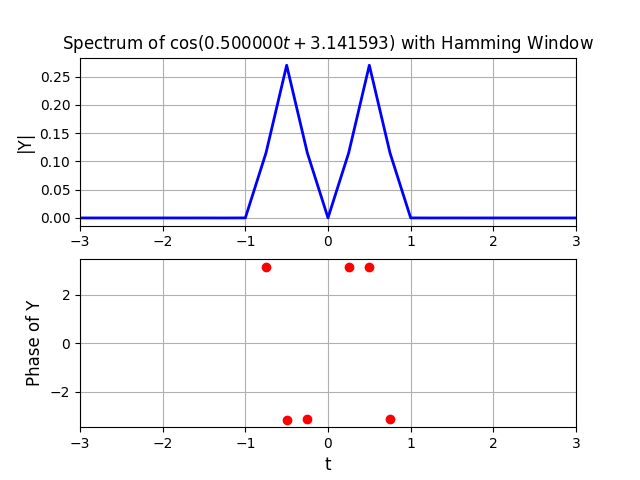
\includegraphics[scale = 0.8]{Figure_11.png}
    \label{fig:sample}
\end{figure}
\begin{center}
    This is the DFT for $\omega_{o} = 0.5$ rad/s and $\delta = \pi$ rad. The peaks are broad as expected.
\end{center}
By using the above mentioned technique for calculating $\omega_{o}$ and $\delta$, I got \textbf{$\omega_{o} = 0.5000072538871699$ and $\delta = 3.141591971950196$} which are close to the actual values of 0.5 and $\pi$.

Now let's assume some white noise (Amplitude=0.1) is present in the signal. This white noise is a gaussian distribution and hence the magnitude doesn't get affected so much. There can be some significant changes in the phase spectrum, but again, the phase values at frequencies $\pm \omega_{o}$ won't get affected very much.
The DFT plot of this noisy signal is:
\begin{figure}[H]
    \centering
    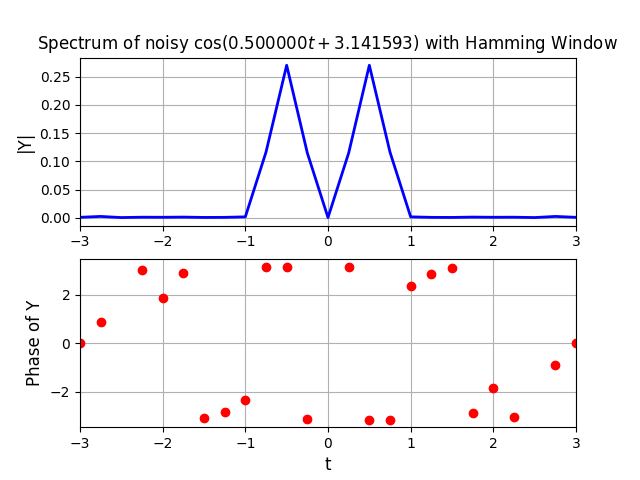
\includegraphics[scale = 0.8]{Figure_12.png}
    \label{fig:sample}
\end{figure}
\begin{center}
    The magnitude plot is a bit noisy by the peaks are still intact. Phase plot also got affected a bit but the overall structure of the plot is preserved
\end{center}
By using the above mentioned technique for calculating $\omega_{o}$ and $\delta$, I got \textbf{$\omega_{o} = 0.5030204449477336$ and $\delta = 3.1357816080573024$} which are close to the actual values of 0.5 and $\pi$.
\subsection{DFT of Chirped Signal}
A chirped signal is a signal whose frequency depends on the time instant. These type of signals will have different frequency components at different time instants. The example given in the assignment is:
\begin{equation*}
    x(t) = \cos(16(1.5 + \frac{t}{2\pi})t)
\end{equation*}
with t ranging from $[-\pi,\pi)$. Also, it is asked to assume $N=1024$. The chirped signal is as shown below:
\begin{figure}[H]
    \centering
    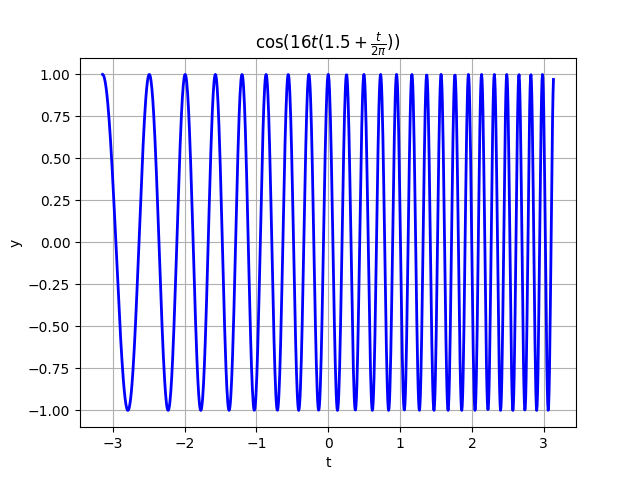
\includegraphics[scale = 0.8]{Figure_13.png}
    \label{fig:sample}
\end{figure}
\begin{center}
    We can observe that the frequency of the chirped signal is changing with time
\end{center}
The DFT of this signal is:
\begin{figure}[H]
    \centering
    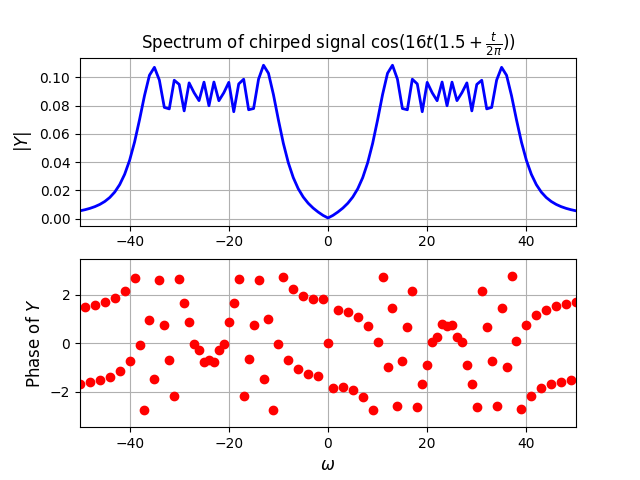
\includegraphics[scale = 0.8]{Figure_14.png}
    \label{fig:sample}
\end{figure}
\begin{center}
    As expected, the signal contains frequency components from $16$ rad/s to $32$ rad/s and the spectrum quickly decays after that range
\end{center}
Now in order to analyze how the frequency comoponents depend on the time range, let us divide the signal into groups of 64 samples. So, we would have 16 such groups. By finding the DFT for each group and plotting the DFT magnitude as a 3d plot with x-axis as time '$t$' and y-axis as frequency '$\omega$', we have the following plot:
\begin{figure}[H]
    \centering
    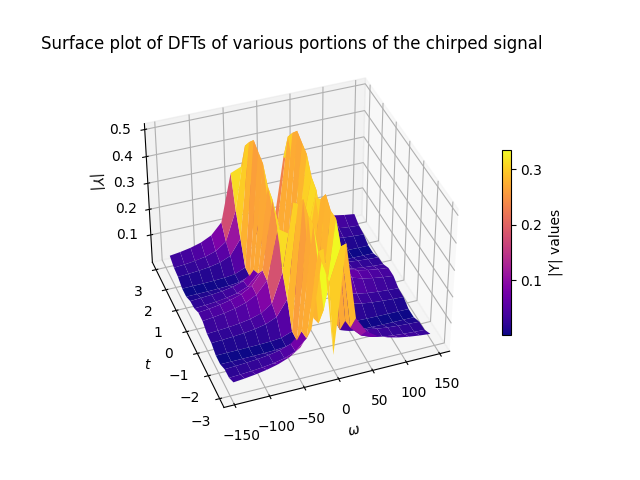
\includegraphics[scale = 0.8]{Figure_15.png}
    \label{fig:sample}
\end{figure}
\begin{center}
    The DFT structure is still the same. However, the peaks are present at different locations depending on the time    
\end{center}
\begin{figure}[H]
    \centering
    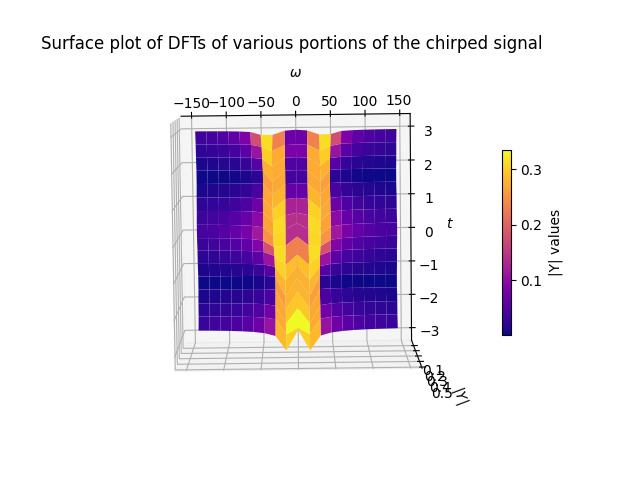
\includegraphics[scale = 0.8]{Figure_16.png}
    \label{fig:sample}
\end{figure}
\begin{center}
    When viewed from above, we can clearly see the peaks widen up indicating the frequencies present in the signal increase with time. Also a linear widening of the peaks mean that the frequencies depend linearly on the time value which is also true
\end{center}
\section{Conclusions}
\begin{enumerate}
    \item When plotting DFT for signals with discontinuities, the spectrum is not
    merely a collection of distinct spikes but a continuous decreasing spectrum
    with $\frac{1}{\omega}$ decay.
    \item To dampen the discontinuities, a Hamming Window is used. This signal is
    multiplied with the original signal so that the high frequency components
    get attenuated and hence, the discontinuities are dampened.
    \item Signal $\cos^{3}(0.86t)$ has a DFT which has broad peaks and continuous decay.
    However, when a hamming window is used, the continuous decay vanishes
    but still the peaks are broad.
    \item To estimate the frequency and initial phase of a sinusoidal signal, its DFT
    is used. The results were fairly accurate when the period of the signal
    is high. White noise didn't affect the results much since its amplitude is
    very low.
    \item The chirped signal has frequency components between 16 rad/s and 32
    rad/s. Also, when the individual DFTs of the 64-samples signals were
    plotted as a function of $\omega$ and $t$, the locations of the peaks widened linearly
    as $t$ increased indicating linear dependence of frequency on $t$.
\end{enumerate}
\end{document}